\documentclass[]{article}

% Imported Packages
%------------------------------------------------------------------------------
\usepackage{amssymb}
\usepackage{amstext}
\usepackage{amsthm}
\usepackage{amsmath}
\usepackage{enumerate}
\usepackage{fancyhdr}
\usepackage[margin=1in]{geometry}
\usepackage{graphicx}
%\usepackage{extarrows}
%\usepackage{setspace}
%\usepackage{xcolor}
\usepackage{color}
\usepackage{parskip}
\usepackage{comment}
\usepackage{enumitem}
\usepackage{hyperref}
%------------------------------------------------------------------------------

% Header and Footer
%------------------------------------------------------------------------------
\pagestyle{plain}  
\renewcommand\headrulewidth{0.4pt}                                      
\renewcommand\footrulewidth{0.4pt}                                    
%------------------------------------------------------------------------------

% Title Details
%------------------------------------------------------------------------------
\title{Deliverable \#1: Software Requirement Specification (SRS)}
\author{SE 3A04: Software Design II -- Large System Design}
\date{}
                            
%------------------------------------------------------------------------------

% Document
%------------------------------------------------------------------------------
\begin{document} 

\maketitle	
\noindent{\bf Tutorial Number:} T03\\
{\bf Group Number:} G8 \\
{\bf Group Members:} Hashim Bukhtiar, Jaden Moore, James Ariache, Olivia Reich, Omar Abdelhamid
\begin{itemize}
        \item Hashim Bukhtiar
        \item Jaden Moore
        \item James Ariache
        \item Olivia Reich
        \item Omar Abdelhamid
\end{itemize}

\section*{IMPORTANT NOTES}
\begin{itemize}
	\item Be sure to include all sections of the template in your document regardless whether you have something to write for each or not
	\begin{itemize}
		\item If you do not have anything to write in a section, indicate this by the \emph{N/A}, \emph{void}, \emph{none}, etc.
	\end{itemize}
	\item Uniquely number each of your requirements for easy identification and cross-referencing
	\item Highlight terms that are defined in Section~1.3 (\textbf{Definitions, Acronyms, and Abbreviations}) with \textbf{bold}, \emph{italic} or \underline{underline}
	\item For Deliverable 1, please highlight, in some fashion, all (you may have more than one) creative and innovative features. Your creative and innovative features will generally be described in Section~2.2 (\textbf{Product Functions}), but it will depend on the type of creative or innovative features you are including.
\end{itemize}

\newpage
\section{Introduction}
\label{sec:introduction}
The SRS is a structured document that outlines the functional and non-functional requirements of the RideRecon software system. It serves as a blueprint for developers, testers, and stakeholders, ensuring a clear understanding of the system to be built. This SRS will provide visibility over software requirements for RideRecon, a car identification application. 
This document will discuss the purpose of RideRecon, the scope of the application, user characteristics, product requirements, and use case diagrams.


\subsection{Purpose}
\label{sub:purpose}
The document focuses on software requirements, user characteristics, and use cases for RideRecon.
The purpose of this SRS is to define the software’s objectives, scope, and functionalities. This document is intended for internal RideRecon stakeholders, including but not limited to, project managers, developers, domain experts, and RideRecon team members/investors. No prior readings are required.

\subsection{Scope}
\label{sub:scope}

RideRecon, the car identification application, will allow users to upload an image and text about a vehicle that they want to identify, consulting up to four “Experts” who will use all or some of the user’s input to determine the make and model of the car that has been depicted.

Users are required to register an account on RideRecon in order to access the car identification service. The service includes four experts: “\underline{RIS}”, “\underline{G8M}”, “\underline{4oE}” and ”\underline{vAI}”. The “\underline{RIS}” expert performs a reverse image search with the user’s given image to identify the car. The “\underline{G8M}” expert is a trained machine learning model by the developers that utilizes an optimized database of car images and their corresponding makes and models to identify the user’s car. The ”\underline{4oE}” expert is the Large Language Model GPT-4o-mini, accessed through OpenAI’s API, which will utilize both the image and the text description to identify the car. Finally, the “\underline{vAI}” expert is also an \underline{LLM}, this one hosted on Google Cloud Platform using Vertex AI, specifically the Gemini 1.0 Flash Model, also accessed through its API.

RideRecon’s objective is not only to identify users’ vehicles, but also to deliver other innovative and creative features. For example, once the car has been identified, \underline{4oE} will provide an interesting fact about the car, adding more depth and intrigue to it, as well as provide sources and listings for where to purchase the car, allowing the user to go one step further and save time if they are interested in making that vehicle their own.

One of the goals of the software is to increase users, as more users will lead to more cars being identified and added to the optimized database of \underline{G8M}, and thus better car identification overall, which is even better for future users. Another goal would be to to monetize its user base by offering premium features like better expert access, exclusive community forums, or partnerships with car-related businesses, thereby creating additional revenue streams beyond the core car identification service. This diversification will improve long-term sustainability and profitability.


\subsection{Definitions, Acronyms, and Abbreviations}
\label{sub:definitions_acronyms_and_abbreviations}
\textbf{LLM}: Large Language Model. A sophisticated artificial intelligence that can understand, generate, and translate human language, often used for tasks like text generation, question answering, and translation.

\textbf{RIS}: Reverse Image Search. This is the idea of using an image as a search query in a browser to find results, rather than using text as traditional browser searches as performed.

\textbf{G8M}: Group 8 Model. This is the model trained by the developers of RideRecon to identify cars. It will utilize an optimized dataset of car images and makes and models.

\textbf{4oE}: GPT-4o-mini. This is an \underline{LLM} that uses text and images to determine the make and model of the user's car.

\textbf{vAI}: Vertex AI, Gemini 1.0 Flash. This is the \underline{LLM} that uses images to determine the make and model of the user's car.

\textbf{Finalizer}: The component of the system that consolidates and finalizes the output, including resolving conflicts between experts and outputting the fun fact about the car and where to purchase it.

\subsection{References}
\label{sub:references}
% Begin SubSection
\iffalse
\begin{itemize}
    \item Provide a complete list of all documents referenced elsewhere in the SRS.
    \item Identify each document by title, report number (if applicable), date, and publishing organization.
    \item Specify the sources from which the references can be obtained.
    \item Order this list in some sensible manner (alphabetical by author, or something else that makes more sense).
\end{itemize}
\fi
\begin{itemize}
    \item[1] “AvtoPix: Car Id - apps on Google Play,” Google, \url{https://play.google.com/store/apps/details?id=ru.egoroffsoft.avtopix&hl=en_CA&pli=1} (accessed Feb. 14, 2025).
    \item[2] “CARSSNAP - car model identify - apps on Google Play,” Google, \url{https://play.google.com/store/apps/details?id=com.mm999.car&hl=en_CA} (accessed Feb. 14, 2025).
    \item[3] Anthony, “Why you should avoid bright, saturated background colors,” UX Movement, \url{https://uxmovement.com/content/why-you-should-avoid-bright-saturated-background-colors/} (accessed Feb. 15, 2025). 
    \item[4] M. Nadir, “Left handedness and mobile user experience,” Medium, \url{https://medium.com/design-bootcamp/left-handedness-and-mobile-user-experience-a3728c72f880} (accessed Feb. 14, 2025).
    \item[5] Written By Jennifer Gaskin  Published: Jan 13, About Jennifer Gaskin      	A veteran of newsrooms and agencies, and A. J. Gaskin, “Color blind design guidelines: A comprehensive guide,” Venngage, \url{https://venngage.com/blog/color-blind-design/} (accessed Feb. 14, 2025).
	\item[6] L. Nikolov, “What’s the difference between API latency and API response time?,” Product Blog Sentry, \url{https://blog.sentry.io/whats-the-difference-between-api-latency-and-api-response-time/#:~:text=Just%20to%20have%20a%20number,to%20abandon%20the%20application%2Fwebsite} (accessed Feb. 15, 2025). 
	\item[7] “Overview of app launch times,” New Relic Documentation, \url{https://docs.newrelic.com/docs/mobile-monitoring/new-relic-mobile/get-started/introduction-app-launch-times/#:~:text=Mobile%20app%20launch%20time%20benchmarks,take%20less%20than%201.5%20seconds} (accessed Feb. 15, 2025).
	\item[8] R. Gordon, “Image recognition accuracy: An unseen challenge confounding today’s AI,” MIT News | Massachusetts Institute of Technology, \url{https://news.mit.edu/2023/image-recognition-accuracy-minimum-viewing-time-metric-1215} (accessed Feb. 15, 2025).
	\item[9] C. Staff, P. Sayer, M. K. Pratt, and M. Bayer, “What is an SLA? Best practices for service-level agreements,” CIO, \url{https://www.cio.com/article/274740/outsourcing-sla-definitions-and-solutions.html} (accessed Feb. 15, 2025).
	\item[10] “How many users is realistic?,” Developer Nation Community, \url{https://www.developernation.net/blog/how-many-users-is-realistic/} (accessed Feb. 15, 2025).
	\item[11] “Implement fallback with API gateway,” API7.ai, \url{https://api7.ai/blog/fallback-api-resilience-design-patterns} (accessed Feb. 15, 2025).
	\item[12] “Amazon S3 pricing - cloud object storage - AWS,” \url{https://aws.amazon.com/s3/pricing/} (accessed Feb. 15, 2025).
	\item[13] IBM, “What is cloud storage?,” IBM, \url{https://www.ibm.com/think/topics/cloud-storage} (accessed Feb. 15, 2025).
	\item[14] IBM, “What is network optimization?,” IBM, \url{https://www.ibm.com/think/topics/network-optimization} (accessed Feb. 15, 2025).
	\item[15] D. S. Sahin Ahmed, “Why does machine learning model performance degrade, and how can we detect and prevent it?,” Medium, \url{https://medium.com/@sahin.samia/why-does-machine-learning-model-performance-degrade-and-how-can-we-detect-and-prevent-it-70f546a54548} (accessed Feb. 15, 2025).
	\item[16] “Adaptive preprocessing and segmentation for a ...,” NDT.net, \url{https://www.ndt.net/article/ctc2012/papers/307.pdf} (accessed Feb. 15, 2025).
	\item[17] F. June, “Model quantization 1: Basic concepts,” Medium, \url{https://medium.com/@florian_algo/model-quantization-1-basic-concepts-860547ec6aa9} (accessed Feb. 15, 2025).
	\item[18] A. Kareliya, “Firebase vs. AWS: Which one to select for your app project in 2025?,” Radixweb, \url{https://radixweb.com/blog/firebase-vs-aws} (accessed Feb. 15, 2025).
	\item[19] “Android 9 PIE: Platform,” Android Developers, \url{https://developer.android.com/about/versions/pie} (accessed Feb. 15, 2025).
	\item[20] “Developer policy center,” Developer Policy Center, \url{https://play.google/developer-content-policy/} (accessed Feb. 15, 2025).
	\item[21] “Privacy checklist  :   android developers,” Android Developers, https://developer.android.com/privacy-and-security/about (accessed Feb. 15, 2025). 
	\item[22] L. S. Branch, “Consolidated federal laws of Canada, Personal Information Protection and Electronic Documents Act,” Personal Information Protection and Electronic Documents Act, \url{https://laws-lois.justice.gc.ca/eng/acts/p-8.6/} (accessed Feb. 15, 2025).
	\item[23] “Legal text,” General Data Protection Regulation (GDPR), \url{https://gdpr-info.eu/} (accessed Feb. 15, 2025).
	\item[24] C. Masha Komnenic CIPP/E, “Mobile app terms and conditions template,” Termly, \url{https://termly.io/resources/templates/app-terms-and-conditions/} (accessed Feb. 15, 2025).
	\item[25] “ISO/IEC 27001:2022,” ISO, \url{https://www.iso.org/standard/27001} (accessed Feb. 15, 2025).
	\item[26] V. Kananda, “What is AES 256 encryption \& how does it work?,” Progress Blogs, \url{https://www.progress.com/blogs/use-aes-256-encryption-secure-data} (accessed Feb. 15, 2025).
	\item[27] “What is OWASP? What is the OWASP Top 10?,” Cloudflare, \url{https://www.cloudflare.com/learning/security/threats/owasp-top-10/} (accessed Feb. 15, 2025).
	\item[28] “Does Canada have a version of the DMCA takedown?,” DMCA Protection \& Takedown Services, \url{https://www.dmca.com/FAQ/Does-Canada-have-a-version-of-the-DMCA-Takedown} (accessed Feb. 15, 2025).

\end{itemize}

% End SubSection

\subsection{Overview}
\label{sub:overview}

\textbf{Section 2} discusses the overall product description talking about the product perspective, product functions, user characteristics, assumptions and dependencies, and apportioning of requirements. 

\textbf{Section 3} contains the Use Case Diagram for the use case scenario of using the RideRecon app. 

\textbf{Section 4} contains the highlights of functional requirements talking about main business events and viewpoints. 

\textbf{Section 5} contains the Non-Functional Requirements talking about Look and Feel Requirements, Usability and Humanity Requirements, Performance Requirements, Operational and Environmental Requirements, Maintainability and Support Requirements, Security Requirements, Cultural and Political Requirements and Legal Requirements. 

Lastly, \textbf{Section A} contains the Division of Labour.


% End Section
\newpage
\section{Overall Product Description}
\label{sec:overall_description}
% Begin Section
\begin{comment}
\begin{itemize}
	\item This section should describe the general factors that affect the product and its requirements. 
	\item It does not state specific requirements.
	\item It provides a \emph{background} for those requirements and makes them easier to understand.
\end{itemize}
\end{comment}

\subsection{Product Perspective}
\label{sub:product_perspective}
% Begin SubSection
\begin{comment}
\begin{itemize}
	\item Put the product into perspective with other related products, i.e., context
	\item If the product is independent and totally self-contained, it should be stated here
	\item If the SRS defines a product that is a component of a larger system, then this subsection should relate the requirements of that larger system to the functionality of the software being developed. Identify interfaces between that larger system and the software to be developed.
	\item A block diagram showing the major components of the larger system, interconnections, and external interfaces can be helpful
\end{itemize}
\end{comment}

RideRecon is a mobile app for car identification that is developed to be compatible with the Android platform.Similar to products such as AvtoPix [1] and CarsSnap [2], it will allow car identification through images while also enhancing search capabilities by also allowing identification through textual descriptions. The product will allow users to create a profile and edit account information linked to that profile. This includes the creation of virtual car collections using car images submitted in the app.

Once an image is selected by the user, the product will have an interface that allows it to interact with different reverse image search technologies. Specifically, it will be able to access a Vertex AI image model and the Reverse Image Search Tool via Google.

If provided textual input by the user, the product will have an interface to interact with Google Search. This interface will also be used to search for relevant car facts that can be returned to the user upon identifying pivotal car identification information.

\begin{center}
	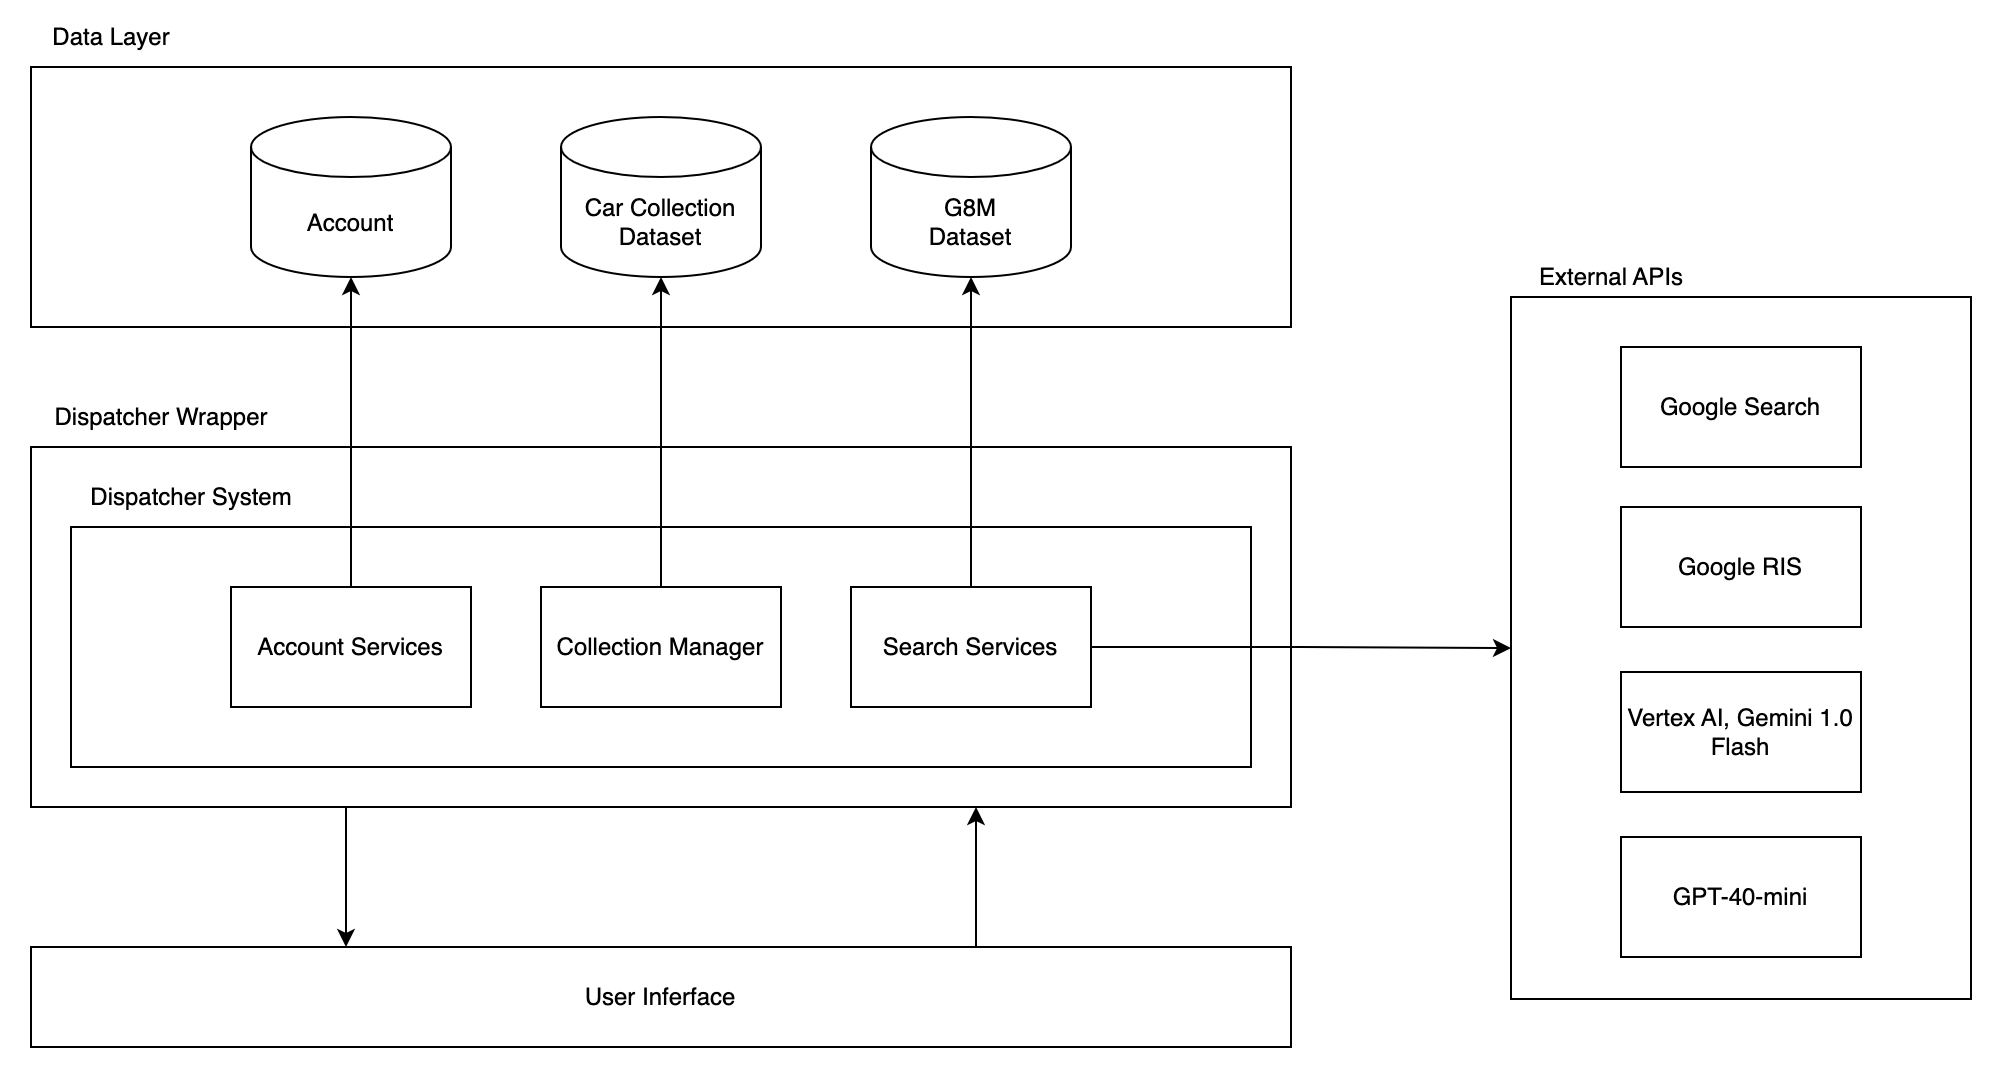
\includegraphics[width=0.9\textwidth]{images/system_diagram.png} \\
	\textbf{Figure 1. } System Diagram
\end{center}

% End SubSection

\newpage
\subsection{Product Functions}
\label{sub:product_functions}
% Begin SubSection
\begin{comment}
\begin{itemize}
	\item Provide a \emph{summary} of the major functions that the software will perform.
	\begin{itemize}
		\item \textbf{Example}: An SRS for an accounting program may use this part to address customer account maintenance, customer statement, and invoice preparation without mentioning the vast amount of detail that each of those functions requires.
	\end{itemize}
	\item Functions should be organized in a way that makes the list of functions understandable to the customer or to anyone else reading the document for the first time 
	\item Present the functions in a list format - each item should be one function, with a brief description of it
	\item Textual or graphical methods can be used to show the different functions and their relationships
	\begin{itemize}
		\item Such a diagram is not intended to show a design of a product, but simply shows the logical relationships among variables
	\end{itemize} 
\end{itemize}
\end{comment}

There will be 3 modules in the product. Each module focuses on different major functions within the product, which have been defined in the table below.

\begin{tabular}{|p{3cm}|p{13cm}|}
	\hline
	Modules & Functions \\
	\hline
	Account Services &
	\begin{itemize} [left=2pt]
		\item Create an account
		\item Login and logout of account
		\item Update account information
		\item Account recovery
		\begin{itemize}
			\item allow user to reset password if forgotten
		\end{itemize}
		\item Authenticate account
		\begin{itemize}
			\item verifies contact information only done during account creation or recovery
		\end{itemize}
	\end{itemize} \\
	\hline
	Search Services &
	\begin{itemize} [left=2pt]
		\item Image search
		\begin{itemize}
			\item allow user to request car identification through an image
		\end{itemize}
		\item Text search
		\begin{itemize}
			\item allow user to request car identification through  text descriptors
		\end{itemize}
		\item Present car information
		\begin{itemize}
			\item displays all relevant identification information
			\item displays ‘fun fact’ information
		\end{itemize}
		\item Confirm car identification
		\begin{itemize}
			\item allow user to confirm whether the identified information matches the car
		\end{itemize}
		\item Add car to collection
		\begin{itemize}
			\item allow user to add identified car to specified ‘Car Collection’
		\end{itemize}
	\end{itemize} \\
	\hline
	Collection Manager &
	\begin{itemize} [left=2pt]
		\item Create new collection
		\begin{itemize}
			\item allow user to create new sub-class in their car collection
		\end{itemize}
		\item View collection
		\begin{itemize}
			\item allow user to select and view a car collection
		\end{itemize}
	\end{itemize} \\
	\hline
\end{tabular}

\begin{center}
	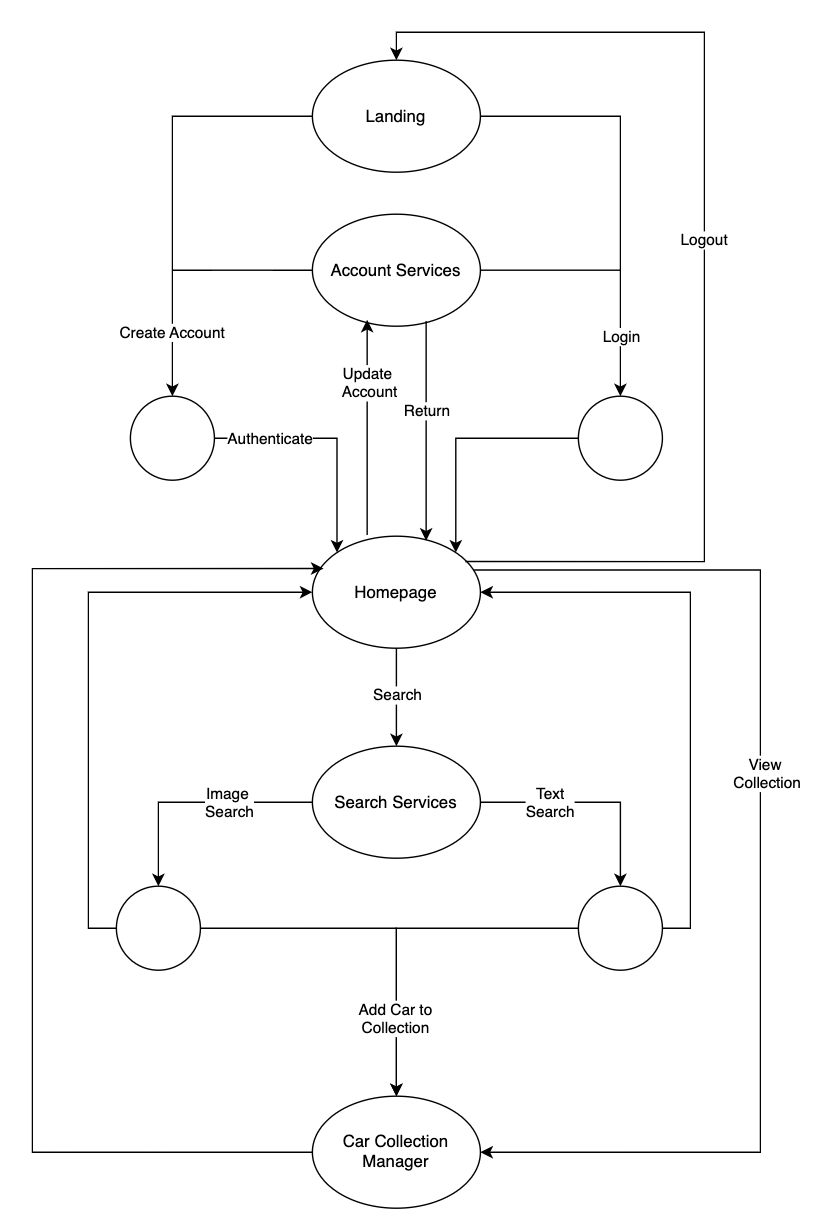
\includegraphics[width=0.5\textwidth]{images/state_diagram.png} \\
	\textbf{Figure 2. } State Diagram
\end{center}
% End SubSection

\subsection{User Characteristics}
\label{sub:user_characteristics}
% Begin SubSection
\begin{comment}
\begin{itemize}
	\item Describe those general characteristics of the intended users of the product including educational level, experience, and technical expertise 
	\item Since there will be many users, you may wish to divide into different user types or personas
%	\item Do not state specific requirements, but rather provide the reasons why certain specific requirements are later specified	
\end{itemize}
\end{comment}
\begin{itemize}
	\item \textbf{Educational Level:} Users must have basic literacy skills which includes the fundamental ability to understand information through reading, writing, listening, and speaking.
	\item \textbf{Technical Expertise:} Users should have a basic understanding of how to operate and navigate an Android smartphone, including downloading apps, as this application is designed specifically for the Android platform.
	\item \textbf{Technical Experience:} Users do not require any prior experience or knowledge with cars in order to utilize the app. Aside from the basic technical expertise outlined above, no extra experience will be required to navigate and utilize the features of the app as it will prioritize an intuitive design.
\end{itemize}
% End SubSection

\subsection{Constraints}
\label{sub:constraints}
% Begin SubSection
\begin{itemize}
	\item Provide a general description of any constraints that will limit the developer's options
	
	\item The system must have an active \textbf{internet connection} to perform car identification.
    \item The app must be compatible with \textbf{Android 9.0 (Pie) and above}.
    \item The device must have at least \textbf{2GB of RAM} for smooth operation.
    \item Captured images must have a \textbf{minimum resolution of 720p} to ensure accurate car identification.
    \item The AI model may not recognize \textbf{damaged or heavily modified cars} accurately.
    \item The system must comply with \textbf{privacy laws} regarding the storage and processing of user-uploaded images.

\end{itemize}
% End SubSection

\subsection{Assumptions and Dependencies}
\label{sub:assumptions_and_dependencies}
% Begin SubSection
\begin{itemize}
\iffalse
	\item List any assumptions you made in interpreting what the software being developed is aiming to achieve
	\item List any other assumptions you made that, if it fails to hold, could require you to change the requirements
	%\item List each of the factors that affect the requirements stated in the SRS
	%\item These factors are not design constraints on the software but are, rather, any changes to them that can affect the requirements in the SRS
	\begin{itemize}
		\item \textbf{Example}: An assumption may be that a specific operating system will be available on the hardware designated for the software product. If, in fact, the operating system is not available, the SRS would then have to change accordingly.
	\end{itemize}
\fi
	\item \textbf{Assumptions:}
    \begin{itemize}
        \item Users will have stable internet access while using the app.
        \item The AI model can identify most common car brands and models.
        \item Dealerships will provide accurate and up-to-date pricing.
    \end{itemize}
    \item \textbf{Dependencies:}
    \begin{itemize}
        \item The AI model relies on an external \textbf{machine learning API} to process images.
        \item The system depends on a third-party \textbf{reverse image search API} (e.g., Google Lens, TinEye) for validation.
        \item Pricing and specifications are sourced from \textbf{external dealership databases}.
    \end{itemize}

\end{itemize}
% End SubSection

\subsection{Apportioning of Requirements}
\label{sub:apportioning_of_requirements}
% Begin SubSection
\textbf{Requirements that may be delayed until future versions of the system:}
\begin{itemize}
	%\item Identify requirements that may be delayed until future versions of the system
	\item \textbf{Offline Mode}: The app currently requires internet access; an offline model will be explored in future versions.
    \item \textbf{Multiple Car Detection}: Initially, the app will support one car per image; future updates may allow multiple cars.
    \item \textbf{Personalized Car Recommendations}: The first version won’t suggest similar cars, but this may be added later.
\end{itemize}
% End SubSection

% End Section
\section{Use Case Diagram}
\label{sec:use_case_diagram}
% Begin Section
\iffalse
\begin{itemize}
	\item Provide the use case diagram for the system being developed.
	\item You do not need to provide the textual description of any of the use cases here (these will be specified under "Highlights of Functional Requirements").
%	\item Provide \emph{one} use case diagram for the most important Business Event.
%	\item The text of all use cases will be specified under "Highlights of Functional Requirements"
\end{itemize}
\fi
\begin{center}
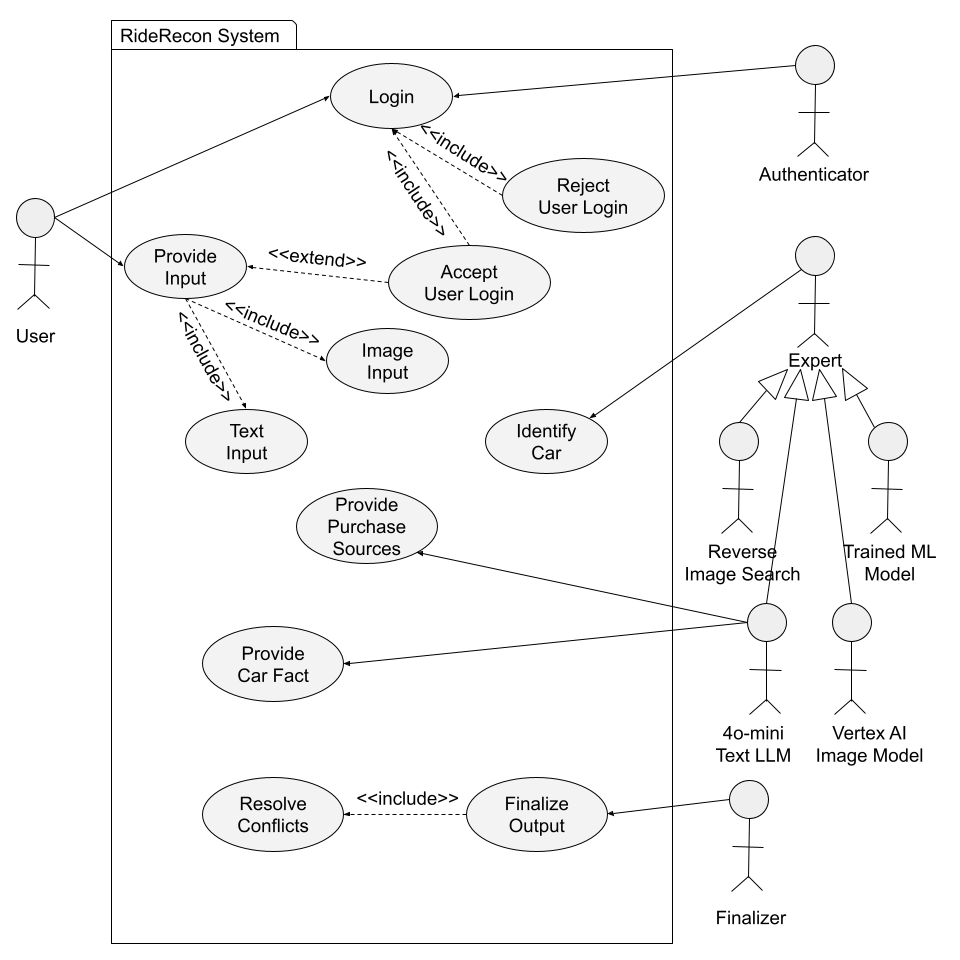
\includegraphics[height=13cm]{images/Use Case Diagram D1.png} \\
\textbf{Figure 3. } Use Case Diagram
\end{center}

%In this section, select the most important Business Event that your system responds to and give its use case diagram.  Only one use case diagram is needed.  Give a brief textual description of the use case without repeating what is in the scenarios of the corresponding Business Event.

%
%
%
%This section should provide a use case diagram for your application. 
%\begin{enumerate}[a)]
%	\item Each use case appearing in the diagram should be accompanied by a text description. 
%\end{enumerate}
%% End Section

\section{Highlights of Functional Requirements}
\label{sec:functional_requirements}
% Begin Section
\iffalse
\begin{itemize}
	\item Specify all use cases (or other scenarios triggered by other events), organized by Business Event. 
	\item For each Business Event, show the scenario from every Viewpoint. You should have the same set of Viewpoints across all Business Events. If a Viewpoint doesn't participate, write N/A so we know you considered it still. You can choose how to present this - keep in mind it should be easy to follow. 
	\item At the end, combine them all into a Global Scenario.
	%\item Specify the "use cases" (or other triggering events) organized by Business Event. (The Global Scenario is what you might think of as a use case). Be sure to consider Business Events that aren't just triggered by users with goals (e.g. something happens in the environment that your system needs to respond to)
	\item Your focus should be on what the system needs to do, not how to do it. Specify it in enough detail that it clearly specifies what needs to be accomplished, but not so detailed that you start programming or making design decisions.
	\item Keep the length of each use case (Global Scenario) manageable. If it's getting too long, split into sub-cases.
	\item You are \emph{not} specifying a complete and consistent set of functional requirements here. (i.e. you are providing them in the form of use cases/global scenarios, not a refined list). For the purpose of this project, you do not need to reduce them to a list; the global scenarios format is all you need.
	\item Red text below is just to highlight where you need to insert a scenario - don't actually write it all in red.
\end{itemize}
\fi
\noindent {\bf Main Business Events:} 
%List out all the main business events you are presenting. If you sub-divided into smaller ones, you don't need to include the smaller ones in this list.\\
\begin{itemize}
        \item BE1. Create Account
        \item BE2. Authenticate User
        \item BE3. Upload Text and/or Image as Input
        \item BE4. Compare Expert Answers
        \item BE5. Present Final Output With Identification Information
        \item BE6. Add to or Remove From Car Collection
\end{itemize}

\noindent {\bf Viewpoints:} 
%List out all the viewpoints you will be considering.\\
\begin{itemize}
	\item VP1. Users
	\item VP2. Customer Support (RideRecon)
	\item VP3. Marketing (RideRecon)
	\item VP4. Accounting (RideRecon)
	\item VP5. Dealership
\end{itemize}

\noindent {\bf Interpretation:} Specify any liberties you took in interpreting business events, if necessary.
\begin{itemize}
	\item NA.
\end{itemize}

\begin{enumerate}[label={\bf BE\arabic*.}]
	\setlist[enumerate]{nosep}
	\item Create an Account \#1\\
	\textbf{Preconditions:} The user is not logged in, thus the log-in screen is displayed
	\begin{enumerate}[label={\bf VP\arabic*.}]		
		\item User \#1\\
		\textbf{Main Success Scenario}
		\begin{enumerate}[label={\arabic*.}]			
			\color{red}
			\item User opens the RideRecon app
			\item The system responds by showing the user the log-in screen interface.
			\item User selects create account
			\item The system displays a screen to request information from the user relating to their account.
			\item The user provides information to make the account and selects the option to confirm the account creation.
			\item The system ensures the user's information is valid and grants them access to the main functionalities of the system.
		\end{enumerate}
		\textbf{Secondary Scenario}
		\begin{enumerate}
			\color{red}
			\item[3i.] User selects "sign in as guest"
			\begin{enumerate}
				\item[3i.1] User selects "sign in as guest"
				\item[3i.2] System grants user access to RideRecon app in guest mode.
			\end{enumerate}
			\item[5i.] User cancels the operation
			\begin{enumerate}
				\item[5i.1] User cancels the operation
				\item[5i.2] System returns them to the log-in menu
			\end{enumerate}													\item[6i.] The system detects the user's information is invalid
			\begin{enumerate}
				\item[6i.1] The system detects the user's information is invalid
				\item[6i.2] The system returns an message to the user stating the information is invalid.
				\item[6i.3] The user acknowledges the message.
				\item[6i.4] The system returns the user to the information request screen in step \textbf{5.}
			\end{enumerate}
			\item[6ii.] An error occurs and the system is unable to validate the user's information.
			\begin{enumerate}
				\item[6ii.1] An error occurs and the system is unable to validate the user's information.
				\item[6ii.2] The system returns an message to the user stating an error has occurred.
				\item[6ii.3] The user acknowledges the error.
				\item[6ii.4] The system returns the user to the information request screen in step \textbf{5.}
			\end{enumerate}
		\end{enumerate}
		\item Customer Support \#2			
			\begin{enumerate}
				\color{red}
%				\item[\textbf{5xi.}] User selects terms of service option to see terms of service.
%				\begin{enumerate}
%					\item[\textbf{5xi.1}] User selects "how to sign up" option to get more information on how to sign up
%					\item[\textbf{5xi.2}] User is redirected to 
%				\end{enumerate}
				\item[5i.] User selects get support option to speak with customer support regarding signup
				\begin{enumerate}
					\item[5i.1] User selects get support option to speak with customer support regarding signup
					\item[5i.2] System redirects the user to a location outside of the app where the user can get in touch with our contractor's customer support line.
				\end{enumerate}
				\item[6i.] An error occurs and the user's information cannot be validated.
				\begin{enumerate}
					\item[6i.1] An error occurs and the user's information cannot be validated.
					\item[6i.2] The system sends a message to the user asking if they want to submit a crash report for analysis.
					\item[6i.3] The user selects yes or no.
					\item[6i.4] If yes is selected, the system sends a crash report of the error to the system maintainers. If no is selected, nothing happens.
					\item[6i.5] The system returns the user to the information request screen in \textbf{step 5.}
				\end{enumerate}
			\end{enumerate}
			\item Marketing \#3\\
			N/A
			\item Accounting \#4\\
			N/A
			\item Dealership \#5\\
			N/A
		\end{enumerate}
		{\bf Global Scenario:}\\
		\textbf{Main Success Scenario}
		\begin{enumerate}[label={\arabic*.}]
			\color{red}
			\item User opens the RideRecon app
			\item The system responds by showing the user the log-in screen interface.
			\item User selects create account
			\item The system displays a screen to request information from the user relating to their account.
			\item The user provides information to make the account and selects the option to confirm the account creation.
			\item The system ensures the user's information is valid and grants them access to the main functionalities of the system.
		\end{enumerate}
		\textbf{Secondary Scenario}
		\begin{enumerate}
			\color{red}
			\item[3i.] User selects "sign in as guest"
			\begin{enumerate}
				\item[3i.1] User selects "sign in as guest"
				\item[3i.2] User gains access to the system in guest mode.  
			\end{enumerate}
			\item[5i.] User cancels the operation
			\begin{enumerate}
				\item[5i.1] User cancels the operation
				\item[5i.2] System returns them to the log-in menu
			\end{enumerate}						
			\item[5ii.] User selects get support option to speak with customer support regarding signup
			\begin{enumerate}
				\item[5ii.1] User selects get support option to speak with customer support regarding signup
				\item[5ii.2] System redirects the user to a location outside of the app where the user can get in touch with our contractor's customer support line.
			\end{enumerate}													\item[6i.] The system detects the user's information is invalid
			\begin{enumerate}
				\item[6i.1] The system detects the user's information is invalid
				\item[6i.2] The system returns an message to the user stating the information is invalid.
				\item[6i.3] The user acknowledges the message.
				\item[6i.4] The system returns the user to the information request screen in step \textbf{5.}				 							\end{enumerate}
			\item[6ii.] An error occurs and the system is unable to validate the user's information.
			\begin{enumerate}
				\item[6ii.1] An error occurs and the system is unable to validate the user's information.
				\item[6ii.2] The system returns an message to the user stating an error has occurred. Alongside the message, the system prompts the user to submit a crash report to the system maintainers for analysis.
				\item[6ii.4] The user selects either yes or no to submitting a crash report.
				\item[6ii.5] If the user selected yes, a crash report of the error is submitted to the system maintainers. If no is selected, nothing happens.
				\item[6ii.6] The system returns the user to the information request screen in step \textbf{5.}
			\end{enumerate}
		\end{enumerate}
	%\end{enumerate}
	\item Authenticate User \#2 \\
	\textbf{Pre-Condition:} The user must have an existing RideRecon account and access to the internet. The system must be able to connect to the authentication server to verify login credentials.
	\begin{enumerate}[label={\bf VP\arabic*.}]
		\item Users \#1 
			\textbf{Main Success Scenario} \\  
			\textcolor{red}{1. User opens the RideRecon app.} \\  
			\textcolor{red}{2. System displays the log-in screen.} \\  
			\textcolor{red}{3. User enters their email/username and password.} \\  
			\textcolor{red}{4. System verifies credentials against the database.} \\  
			\textcolor{red}{5. If credentials are valid, the system grants access to the user and loads the homepage.} \\

			\textbf{Secondary Scenario} \\
            \textcolor{red}{4i. User enters incorrect credentials.} \\  
            \textcolor{red}{4ii. System detects invalid credentials and displays an error message.} \\  
            \textcolor{red}{4iii. User is given the option to retry or reset their password.} \\  
            \textcolor{red}{4iv. If the user retries, they are redirected back to the login screen.} \\  
            \textcolor{red}{4v. If the user selects password reset, they are taken to the password recovery process.} \\  
            \textcolor{red}{5i. System is unable to connect to the authentication server.} \\  
            \textcolor{red}{5ii. System displays a message informing the user of a connection issue.} \\  
            \textcolor{red}{5iii. User is given the option to retry logging in.} \\  
            \textcolor{red}{6i. User selects "Remember Me" during login.} \\  
            \textcolor{red}{6ii. System securely stores authentication tokens to allow automatic login on future app openings.} \\  
            \textcolor{red}{7i. User selects "Sign in with Google/Apple ID".} \\  
            \textcolor{red}{7ii. System redirects user to the respective authentication service.} \\  
            \textcolor{red}{7iii. If authentication is successful, user is granted access to the app.} \\ 
		\item Customer Support (RideRecon) \#2 \\
			\textbf{Main Success Scenario} \\  
			\textcolor{red}{1. User selects the "Need Help?" option on the login screen.} \\  
			\textcolor{red}{2. System displays support options, including FAQs and a contact form.} \\  
			\textcolor{red}{3. User submits an inquiry regarding login issues.} \\  
			\textcolor{red}{4. System sends the inquiry to customer support.} \\  
			
			\textbf{Secondary Scenario}  
			\textcolor{red}{4i. System provides automated troubleshooting suggestions before allowing the user to submit a ticket.} \\  
			\textcolor{red}{4ii. If an error prevents login, system suggests clearing cache or checking for updates.} \\ 
		\item Marketing (RideRecon) \#3 \\
			\textcolor{red}{N/A}
		\item Accounting (RideRecon) \#4 \\
			\textcolor{red}{N/A}
		\item Dealership \#5 \\
			\textcolor{red}{N/A}
	\end{enumerate}	
	{\bf Global Scenario:}\\
	\textbf{Main Success Scenario} \\  
	\textcolor{red}{1. User opens the RideRecon app.} \\  
	\textcolor{red}{2. System displays the log-in screen.} \\  
	\textcolor{red}{3. User enters login credentials.} \\  
	\textcolor{red}{4. System verifies credentials.} \\  
	\textcolor{red}{5. If valid, user is granted access to the app.} \\ 

	\textbf{Secondary Scenario} \\  
	\textcolor{red}{4i. User enters incorrect credentials and is prompted to retry or reset their password.} \\  
	\textcolor{red}{4ii. System encounters a connectivity issue and informs the user.} \\  
	\textcolor{red}{4iii. User opts to remember their credentials for future logins.} \\  
	\textcolor{red}{4iv. User logs in using third-party authentication (Google/Apple ID).} \\

	\item Upload Text and/or Image as Input \#3 \\  
    \textbf{Pre-Condition:} The user must be authenticated in the system and must have an active internet connection. The user must either provide an image of the car or enter a textual description. If using an image, the device must have a functioning camera or access to stored images.
  

    \begin{enumerate}[label=\textbf{VP\arabic*.}]
        \item Users \#1 \\  
            \textbf{Main Success Scenario} \\  
            \textcolor{red}{1. The user selects an image OR enters text describing a car.} \\  
            \textcolor{red}{2. If an image is provided, the system checks its quality:
			If acceptable, the system processes the image.
			If blurry, the system prompts the user to retake the photo.} \\  
            \textcolor{red}{3. If text is provided, the system extracts key information and performs a database search.} \\  
            \textcolor{red}{4. The system provides instant feedback while processing.} \\  
            \textcolor{red}{5. The user receives results, including car specifications and pricing (if available).} \\  
            \textcolor{red}{6. The system sends the input data to the Experts for processing.} \\  
            
            \textbf{Secondary Scenario} \\  
            \textcolor{red}{6i. User provides an image, but it is blurry or unclear.} \\  
            \textcolor{red}{6ii. System detects poor image quality and prompts the user to re-upload a clearer image.} \\  
            \textcolor{red}{6iii. User does not have an image and enters text instead.} \\  
            \textcolor{red}{6iv. System prompts the user to refine their text description if it is too vague.} \\  
            \textcolor{red}{6v. The Experts detect that the provided image and text do not match the same car model.} \\  
            \textcolor{red}{6vi. System prompts the user to confirm or edit the text description to match the uploaded image.} \\  

        \item Customer Support (RideRecon) \#2 \\  
            \textcolor{red}{NA}  

        \item Marketing (RideRecon) \#3 \\  
            \textcolor{red}{NA}  

        \item Accounting (RideRecon) \#4 \\  
            \textcolor{red}{NA}  

        \item Dealership \#5 \\  
            \textcolor{red}{9i. The system determines that the dealership database lacks a match for the provided input.} \\  
            \textcolor{red}{9ii. The dealership can request to update the system database to ensure their listings appear in future searches.} \\
	\end{enumerate}

	{\bf Global Scenario:} \\  
		\textbf{Main Success Scenario} \\  
		\textcolor{red}{1. User opens the RideRecon app on their device.} \\  
		\textcolor{red}{2. System requires the user to log in and displays the login fields.} \\  
		\textcolor{red}{3. User enters login credentials.} \\  
		\textcolor{red}{4. System authenticates the user.} \\  
		\textcolor{red}{5. System prompts the user to upload an image or enter a text description of the car they want to identify.} \\  
		\textcolor{red}{6. User uploads an image or enters a text description.} \\  
		\textcolor{red}{7. System verifies the uploaded image quality and processes it.} \\  
		\textcolor{red}{8. System processes the text description using language processing and matches potential vehicles.} \\  
		\textcolor{red}{9. System sends the input data to the Experts for processing.} \\  

		\textbf{Secondary Scenario} \\  
		\textcolor{red}{6i. User provides an image, but it is blurry or unclear.} \\  
		\textcolor{red}{6ii. System detects poor image quality and prompts the user to re-upload a clearer image.} \\  
		\textcolor{red}{6iii. User does not have an image and enters text instead.} \\  
		\textcolor{red}{6iv. System prompts the user to refine their text description if it is too vague.} \\  
		\textcolor{red}{9i. The Experts detect that the provided image and text do not match the same car model.} \\  
		\textcolor{red}{9ii. System prompts the user to confirm or edit the text description to match the uploaded image.} \\  

	\item Compare Expert Answers \#4
	\begin{enumerate}[label={\bf VP\arabic*.}]
		\item User \#1\\
		\textbf{Main Success Scenario}
		\begin{enumerate}[label={\arabic*.}]
			\color{red}
			\item User provides the information of a car for the system to process.
			\item System feeds input to all of its experts
			\item Experts provide the system with their answer on information about the car.
			\item The \underline{Finalizer} recognizes the experts agree on what kind of car the user inputs.
			\item The \underline{Finalizer} processes the data from the experts for output.
		\end{enumerate}
		\textbf{Secondary Scenario}
		\begin{enumerate}
			\color{red}
			\item[4i.] The \underline{Finalizer} recognizes that not all of the experts agree on what kind of car has been input into the system.
			\begin{enumerate}
				\item[4i.1] The \underline{Finalizer} recognizes that not all of the experts agree on what kind of car has been input into the system.
				\item[4i.2] Using conflict resolution methods, the \underline{Finalizer} will determine which experts to accept information from.
				\item[4i.3] If a certain threshold of certainty is reached by the \underline{Finalizer}, the \underline{Finalizer} will use information from the selected experts in output processing. If not, the system will attempt to provide information to the experts that will refine their outputs and the system returns to step  \textbf{3.} in the process.
				\item[4i.4] After a pre-defined maximum amount of attempts to refine the solution is reached, the system will notify the user that it was unable to find the car that was input.
				\item[4i.5] The user acknowledges the message.
				\item[4i.6] The system returns itself to the state where the user can provide input for identifying a car.
			\end{enumerate}
		\end{enumerate}
		\item Customer Support \#2
		\begin{enumerate}
			\color{red}
			\item[4i.] Should the experts and \underline{Finalizer} fail to determine what car was input by the user, the system will prompt the user with the option to send feedback.
			\begin{enumerate}
				\item[4i.1] Should the experts and \underline{Finalizer} fail to determine what car was input by the user, the system will prompt the user with the option to send feedback.
				\item[4i.2] The user can select yes or no to this prompt.
				\item[4i.3] If the user selects no, nothing happens and the system is returned to a state where the user can provide input for identifying a car again. If the user selects yes, the system will prompt them for their feedback and any other important information.
				\item[4i.4] The user inputs their feedback.
				\item[4i.5] The system thanks the user for their feedback and returns them to a state where they can provide input for identifying a car again.
			\end{enumerate}
		\end{enumerate}
		\item Marketing\\
		N/A
		\item Accounting\\
		N/A
		\item Dealership\\
		N/A
		\end{enumerate}
		{\bf Global Scenario:}\\
		\textbf{Main Success Scenario}
		\begin{enumerate}[label={\arabic*.}]
			\color{red}
			\item User provides the information of a car for the system to process.
			\item System feeds input to all of its experts
			\item Experts provide the system with their answer on information about the car.
			\item The \underline{Finalizer} recognizes the experts agree on what kind of car the user inputs.
			\item The \underline{Finalizer} processes the data from the experts for output.
		\end{enumerate}
		\textbf{Secondary Scenario}
		\begin{enumerate}
			\color{red}
			\item[4i.] The \underline{Finalizer} recognizes that not all of the experts agree on what kind of car has been input into the system.
			\begin{enumerate}
				\item[4i.1] The \underline{Finalizer} recognizes that not all of the experts agree on what kind of car has been input into the system.
				\item[4i.2] Using conflict resolution methods, the \underline{Finalizer} will determine which experts to accept information from.
				\item[4i.3] If a certain threshold of certainty is reached by the \underline{Finalizer}, the \underline{Finalizer} will use information from the selected experts in output processing. If not, the system will attempt to provide information to the experts that will refine their outputs and the system returns to step  \textbf{3.} in the process.
				\item[4i.4] After a pre-defined maximum amount of attempts to refine the solution is reached, the system will notify the user that it was unable to find the car that was input. Alongside this message will be an option to send feedback to the system maintainers about the experience.
				\item[4i.5] The user acknowledges the message and chooses not to give feedback.
				\item[4i.5.i.1] The user decides to give feedback.
				\item[4i.5.i.2] The system will prompt the user for their feedback and any other important information.
				\item[4i.5.i.3] The user inputs their feedback.
				\item[4i.5.i.4] The system thanks them for their response.
				\item[4i.6] The system returns itself to the state where the user can provide input for identifying a car.
			\end{enumerate} 
		\end{enumerate}
	%\end{enumerate}
\item Finalize and Present Output With Identification Information \#5 \\
		\textbf{Pre-Condition:} All experts have processed input and obtained their final answer for the make and model of the car.
		\begin{enumerate}[label=\textbf{VP\arabic*.}]
			\item Users \#1 \\
				\textbf{Main Success Scenario} \\
				\textcolor{red}{1. User opens the RideRecon app on their device.} \\
				\textcolor{red}{2. System requires the user to log in and displays the login fields.} \\
				\textcolor{red}{3. User enters login credentials.} \\
				\textcolor{red}{4. System authenticates the user.} \\
				\textcolor{red}{5. System prompts the user to upload an image and text description of the car they want to identify.} \\
				\textcolor{red}{6. User uploads an image with some text description of their car.} \\
				\textcolor{red}{7. The input data is sent to the Experts for processing.} \\
				\textcolor{red}{8. All Experts come to the same conclusion about the make and model of the car.} \\
				\textcolor{red}{9. The \underline{Finalizer} displays the make and model of the car, as well as the fun fact and where to purchase the car.} \\
				\textbf{Secondary Scenario} \\
				\textcolor{red}{6i. User doesn't have both forms of input.} \\
				\textcolor{red}{6ii. System prompts the user to provide the missing form of input.} \\
				\textcolor{red}{6iii. Available form of input is given to the Expderts which will do their best to determine the car.} \\
				\textcolor{red}{8i. The Experts come to different conclusions about the make and model of the car.} \\
				\textcolor{red}{9i. The \underline{Finalizer} displays all Expert answers, with a recommendation on which is most likely based on how many Experts came to the same conclusion.} \\
				\textcolor{red}{9ii. The \underline{Finalizer} also obtains fun facts and purchase information about ALL cars that the Experts concluded on.} \\
			\item Customer Support (RideRecon) \#2 \\
				\textcolor{red}{NA}
			\item Marketing (RideRecon) \#3 \\
				\textcolor{red}{NA}
			\item Accounting (RideRecon) \#4 \\
				\textcolor{red}{NA}
			\item Dealership \#5 \\
				\textcolor{red}{9i. The given dealership was not chosen as a source of purchase.} \\
				\textcolor{red}{9ii. They can contact RideRecon to ensure that they are more likely to be chosen as the preferred purchase source.}

		\end{enumerate}
		{\bf Global Scenario:}\\
			\textbf{Main Success Scenario} \\
			\textcolor{red}{1. User opens the RideRecon app on their device.} \\
			\textcolor{red}{2. System requires the user to log in and displays the login fields.} \\
			\textcolor{red}{3. User enters login credentials.} \\
			\textcolor{red}{4. System authenticates the user.} \\
			\textcolor{red}{5. System prompts the user to upload an image and text description of the car they want to identify.} \\
			\textcolor{red}{6. User uploads an image with some text description of their car.} \\
			\textcolor{red}{7. The input data is sent to the Experts for processing.} \\
			\textcolor{red}{8. All Experts come to the same conclusion about the make and model of the car.} \\
			\textcolor{red}{9. The \underline{Finalizer} displays the make and model of the car, as well as the fun fact and where to purchase the car.} \\
			\textbf{Secondary Scenario} \\
			\textcolor{red}{6i. User doesn't have both forms of input.} \\
			\textcolor{red}{6ii. System prompts the user to provide the missing form of input.} \\
			\textcolor{red}{6iii. Available form of input is given to the Expderts which will do their best to determine the car.} \\
			\textcolor{red}{8i. The Experts come to different conclusions about the make and model of the car.} \\
			\textcolor{red}{9i. The \underline{Finalizer} displays all Expert answers, with a recommendation on which is most likely based on how many Experts came to the same conclusion.} \\
			\textcolor{red}{9ii. The \underline{Finalizer} also obtains fun facts and purchase information about ALL cars that the Experts concluded on.} \\
			
	\item Add to Car Collection \#6 \\
	\textbf{Pre-Condition:} The user must be logged into their account.
	\begin{enumerate}[label=\textbf{VP\arabic*.}]
		\item Users \#1 \\
		\textbf{Main Success Scenario} \\
		1. User accesses their car collections through the icon on the homepage. \\
		2. User chooses the add to car collection icon. \\
		3. System prompts the user to choose a car from their past identification history. \\
		4. User selected an identified car. \\
		5. System prompts the user to choose a car collection. \\
		6. User selects an existing car collection to add the identified car to. \\
		7. The input data is sent to the Experts for processing. \\
		8. System provides a review of changes to car collection and prompts the user for verification. \\
		9. User verifies changes and returns to homepage. \\
		\textbf{Secondary Scenario} \\
		1i. User chooses to add a car to a collection immediately after identification. Skip VP1.2 \& VP1.3. \\
		2i. No past identified car. Return to homepage. \\
		8i. User declines changes. No modification made to car collection and return to homepage. \\
		\item Customer Support (RideRecon) \#2 \\
		\textcolor{red}{NA}
		\item Marketing (RideRecon) \#3 \\
		\textcolor{red}{NA}
		\item Accounting (RideRecon) \#4 \\
		\textcolor{red}{NA}
		\item Dealership \#5 \\
		\textcolor{red}{NA}
	\end{enumerate}
	{\bf Global Scenario:}\\
	\textbf{Main Success Scenario} \\
	1. User accesses their car collections through the icon on the homepage. \\
	2. User chooses the add to car collection icon. \\
	3. System prompts the user to choose a car from their past identification history. \\
	4. User selected an identified car. \\
	5. System prompts the user to choose a car collection. \\
	6. User selects an existing car collection to add the identified car to. \\
	7. The input data is sent to the Experts for processing. \\
	8. System provides a review of changes to car collection and prompts the user for verification. \\
	9. User verifies changes and returns to homepage. \\
	\textbf{Secondary Scenario} \\
	1i. User chooses to add a car to a collection immediately after identification. Skip VP1.2 \& VP1.3. \\
	2i. No past identified car. Return to homepage. \\
	8i. User declines changes. No modification made to car collection and return to homepage. \\
\end{enumerate}

%	Below, we organize by Business Event.
%	\begin{enumerate}[{BE}1.]
%		\item Business Event name
%		\begin{enumerate}[{VP1}.1]
%			\item Viewpoint name \newline
%			\noindent\fbox{%
%				\parbox{0.5\textwidth}{%
%					\begin{itemize}
%						\item {\bf $S_{1}$:} Initial response of the system to the Business Event
%						\item {\bf $E_{1}$:}  Reaction of the environment to $S_{1}$
%						\item {\bf $S_{2}$:}  Response of the system to $E_{1}$
%						\item {\bf $E_{2}$:}  Reaction of the environment to $S_{2}$
%						\item[] $\cdots$
%						\item {\bf $S_{n}$:}  Response of the system to $E_{(n-1)}$
%						\item {\bf $E_{n}$:}  Reaction of the environment to $E_{(n-1)}$
%						\item {\bf $S_{(n+1)}$:} Final response of the system concluding its function regarding the Business Event
%					\end{itemize}
%				}%
%			}
%			\item Viewpoint name\newline
%			\noindent\fbox{%
%				\parbox{0.5\textwidth}{%
%					\begin{itemize}
%						\item {\bf $S_{1}$:} Initial response of the system to the Business Event
%						\item {\bf $E_{1}$:}  Reaction of the environment to $S_{1}$
%						\item {\bf $S_{2}$:}  Response of the system to $E_{1}$
%						\item {\bf $E_{2}$:}  Reaction of the environment to $S_{2}$
%						\item[] $\cdots$
%						\item {\bf $S_{k}$:}  Response of the system to $E_{(k-1)}$
%						\item {\bf $E_{k}$:}  Reaction of the environment to $E_{(k-1)}$
%						\item {\bf $S_{(k+1)}$:} Final response of the system concluding its function regarding the Business Event
%					\end{itemize}
%				}%
%			}
%			\item \dots
%			\item \dots
%			\item \dots
%			\item[\dots]
%		\end{enumerate}	
%		\item[] {\bf Global Scenario of {\it Business Event Name}:} It is the scenario corresponding to the integration of all the above scenarios from the different Viewpoints of the Business Event BE1.\newline
%		\noindent\fbox{%
%			\parbox{0.5\textwidth}{%
%				\begin{itemize}
%					\item {\bf $S_{1}$:} Initial response of the system to the Business Event
%					\item {\bf $E_{1}$:}  Reaction of the environment to $S_{1}$
%					\item {\bf $S_{2}$:}  Response of the system to $E_{1}$
%					\item {\bf $E_{2}$:}  Reaction of the environment to $S_{2}$
%					\item[] $\cdots$
%					\item {\bf $S_{m}$:}  Response of the system to $E_{(m-1)}$
%					\item {\bf $E_{m}$:}  Reaction of the environment to $E_{(m-1)}$
%					\item {\bf $S_{(m+1)}$:} Final response of the system concluding its function regarding the Business Event
%				\end{itemize}
%			}%
%		}	
%		%\end{enumerate}
%		\item Business Event name
%		\begin{enumerate}[{VP1}.1]
%			\item Viewpoint name \newline
%			\noindent\fbox{%
%				\parbox{0.5\textwidth}{%
%					\begin{itemize}
%						\item {\bf $S_{1}$:} Initial response of the system to the Business Event
%						\item {\bf $E_{1}$:}  Reaction of the environment to $S_{1}$
%						\item {\bf $S_{2}$:}  Response of the system to $E_{1}$
%						\item {\bf $E_{2}$:}  Reaction of the environment to $S_{2}$
%						\item[] $\cdots$
%						\item {\bf $S_{n'}$:}  Response of the system to $E_{(n'-1)}$
%						\item {\bf $E_{n'}$:}  Reaction of the environment to $E_{(n'-1)}$
%						\item {\bf $S_{(n'+1)}$:} Final response of the system concluding its function regarding the Business Event
%					\end{itemize}
%				}%
%			}
%			\item Viewpoint name\newline
%			\noindent\fbox{%
%				\parbox{0.5\textwidth}{%
%					\begin{itemize}
%						\item {\bf $S_{1}$:} Initial response of the system to the Business Event
%						\item {\bf $E_{1}$:}  Reaction of the environment to $S_{1}$
%						\item {\bf $S_{2}$:}  Response of the system to $E_{1}$
%						\item {\bf $E_{2}$:}  Reaction of the environment to $S_{2}$
%						\item[] $\cdots$
%						\item {\bf $S_{k'}$:}  Response of the system to $E_{(k'-1)}$
%						\item {\bf $E_{k'}$:}  Reaction of the environment to $E_{(k'-1)}$
%						\item {\bf $S_{(k'+1)}$:} Final response of the system concluding its function regarding the Business Event
%					\end{itemize}
%				}%
%			}
%			\item \dots
%			\item \dots
%			\item \dots
%			\item[\dots]
%		\end{enumerate}	
%		\item[] {\bf Global Scenario of {\it Business Event Name}:} It is the scenario corresponding to the integration of all the above scenarios from the different Viewpoints of the Business Event BE2.\newline
%		\noindent\fbox{%
%			\parbox{0.5\textwidth}{%
%				\begin{itemize}
%					\item {\bf $S_{1}$:} Initial response of the system to the Business Event
%					\item {\bf $E_{1}$:}  Reaction of the environment to $S_{1}$
%					\item {\bf $S_{2}$:}  Response of the system to $E_{1}$
%					\item {\bf $E_{2}$:}  Reaction of the environment to $S_{2}$
%					\item[] $\cdots$
%					\item {\bf $S_{m'}$:}  Response of the system to $E_{(m'-1)}$
%					\item {\bf $E_{m'}$:}  Reaction of the environment to $E_{(m'-1)}$
%					\item {\bf $S_{(m'+1)}$:} Final response of the system concluding its function regarding the Business Event
%				\end{itemize}
%			}%
%		}		
%	\end{enumerate}

%End Section

\section{Non-Functional Requirements}
\label{sec:non-functional_requirements}
\iffalse

\begin{itemize}
	\item For each non-functional requirement, provide a justification/rationale for it.\\
	{\bf Example:} \\
	SC1. \emph{The device should not explode in a customer’s pocket.}\\
	{\bf Rationale:} Other companies have had issues with the batteries they used in their phones randomly exploding [insert citation]. This causes a safety issue, as the phone is often carried in a person's hand or pocket.	
	\item If you need to make a guess because you couldn't really talk to stakeholders, you can say "We imagined stakeholders would want...because..."
	\item Each requirement should have a unique label/number for it.
	\item In the list below, if a particular section doesn't apply, just write N/A so we know you considered it.
\end{itemize}
\fi
% Begin Section
\subsection{Look and Feel Requirements}
\label{sub:look_and_feel_requirements}
% Begin SubSection

\subsubsection{Appearance Requirements}
\label{ssub:appearance_requirements}
% Begin SubSubSection
\begin{enumerate}[label={LF-A\arabic*.}]
	\item The system's user interface must use the contractor's colours that align with the ones used in their branding.\\
	\textbf{Rationale:} The user should feel as if the application is closely tied to our contractor and their mission statements.
	\item The system's user interface should not use harsh and overly saturated colours.\\
	\textbf{Rationale:} If the user interface is too bright or saturated, it can strain the user's eyes and users will not want to spend an extended period of time looking at the application[3]. 
	\item The application should be consistent in how it associates colours with certain buttons or actions.\\
	\textbf{Rationale:} When a user goes to do actions across the application, the colour of buttons relating to certain prompts like "yes" or "no" should remain consistent across all of those prompts. For example, if a "yes" button uses the colour green, then any other time "yes" comes up it should also be green.
	\item Users should be able to quickly distinguish what is and what is not a button.\\
	\textbf{Rationale:} The user should be able to quickly understand the options available to them without needing a lot of effort or research. 
\end{enumerate}
% End SubSubSection

\subsubsection{Style Requirements}
\label{ssub:style_requirements}
% Begin SubSubSection
\begin{enumerate}[label={LF-S\arabic*.}]
	\item The system must scale its UI so that it can fit to the size of the screen device.\\
	\textbf{Rationale:} Device screens come in all shapes and sizes, thus the application should be able accommodate all kinds of screen sizes.
	\item Additional options or menus should be hidden under one to a small handful of dropdown menus.\\
	\textbf{Rationale:} The user's screen should not be cluttered with an abundance of buttons that makes the application hard to navigate.
	\item The system should adhere to general practices for making applications for android devices.\\
	\textbf{Rationale:} Since the system is made for android devices, we need to follow general practices for making android applications to fit with the styles of other android applications.
	\item When an expert is mentioned in the system, if it was called by an API call, the system should use the expert's branding appearance when displaying information from it.\\
	\textbf{Rationale:} When a user interacts with the system in a way that displays information from the experts, if the branding from the given expert is used, it will be easily identifiable by the user and will help them gain trust in the information they are receiving.
%	\item On system startup, if the user is logged in, the system should display the frame that allows the user to identify a car.\\
%	\textbf{Rationale:} The system should display the frame that highlights its main functionality to communicate the intended purpose of the system.

\end{enumerate}
% End SubSubSection

% End SubSection

\subsection{Usability and Humanity Requirements}
\label{sub:usability_and_humanity_requirements}
% Begin SubSection

\subsubsection{Ease of Use Requirements}
\label{ssub:ease_of_use_requirements}
% Begin SubSubSection
\begin{enumerate}[label={UH-EOU\arabic*.}]
	\item The system should only require a maximum of two inputs from the user to produce an output.\\
	\textbf{Rationale:} The user should not need to go through an extensive process to identify a car. They should be able to take a picture, type in a model, etc. and receive the results they are looking for.
	\item The system should be usable with only one hand.\\
	\textbf{Rationale:} There are many times in a user's daily life where only one hand is available to them. Thus, making the app usable with only one hand means users would be able to use the app even in those moments.
\end{enumerate}
% End SubSubSection

\subsubsection{Personalization and Internationalization Requirements}
\label{ssub:personalization_and_internationalization_requirements}
% Begin SubSubSection
\begin{enumerate}[label={UH-PI\arabic*.}]
	\item The system should have a variety of language options to choose from.\\
	\textbf{Rationale:} With a variety of users comes a variety of languages that are spoken. Thus, to improve the user's experience, we should give them a wide range of languages to choose from do they can use the app with the language they are most comfortable with.
	\item The system should be easy to use by both right and left handed people.\\
	\textbf{Rationale:} Users have a preference whether to use their phone with their left or right hand, thus the system should be comfortable to use regardless of which hand is used. Furthermore, there are occasions when users are not able to use one hand or the other, so making the application only feel comfortable to use with a specific hand could make the application feel unwieldy [4].
	\item The system should be usable on a lower device brightness.\\
	\textbf{Rationale:} Users will not always have their device at full brightness, so if the device becomes harder to use at these low brightness settings the user will find the system more tedious to work with.
\end{enumerate}

% End SubSubSection

\subsubsection{Learning Requirements}
\label{ssub:learning_requirements}
% Begin SubSubSection
% Mention modern conventions
\begin{enumerate}[label={UH-L\arabic*.}]
	\item Users should be able to start identifying a car within their first 5 minutes of logging into the application.\\
	\textbf{Rationale:} The process of inputting the information required to identify a car should be minimal and should not be complex. Since coming across a car may be a quick experience, it should not take the user a long time to learn how to use the system effectively.
\end{enumerate}
% End SubSubSection

\subsubsection{Understandability and Politeness Requirements}
\label{ssub:understandability_and_politeness_requirements}
% Begin SubSubSection
\begin{enumerate}[label={UH-UP\arabic*.}]
	\item Any icons used in the system without explanation should be universally understood by users or easy to learn.\\
	\textbf{Rationale:} An icon that can be quickly understood or universally known will make it easier for users to understand what our system does.
\end{enumerate}
% End SubSubSection

\subsubsection{Accessibility Requirements}
\label{ssub:accessibility_requirements}
% Begin SubSubSection
\begin{enumerate}[label={UH-A\arabic*.}]
	\item The system should be able to accommodate users with colour blindness.\\
	\textbf{Rationale:} Approximately 360 Million people are colourblind [5]. Thus, as to not alienate a large demographic of users, the interface should be designed with these users in mind.
	\item The system should be compatible with accessibility screen readers.\\
	\textbf{Rationale:} Users with vision or comprehension disabilities might use screen readers to better navigate the devices and applications that they are engaging with. Thus, to make the system accessible to those users it would be necessary to make the system friendly to common screen readers.
\end{enumerate}
% End SubSubSection

% End SubSection

\subsection{Performance Requirements}
\label{sub:performance_requirements}
% Begin SubSection

\subsubsection{Speed and Latency Requirements}
\label{ssub:speed_and_latency_requirements}
% Begin SubSubSection
\begin{enumerate}[label={PR-SL\arabic*.}]
    \item The response time of all core APIs should be under 1 second for 90\% of requests and must not exceed 5 seconds.\\ 
	\textbf{Rationale:} Research on mobile application UX shows that users expect instantaneous responses, with 1 second or less considered a high-performing API response time. At 2 seconds, delays become noticeable, and beyond 5 seconds, users are likely to abandon the interaction or log off the app[6].
	\item A cold start (first launch or after app closure) must be under 5 seconds, while a hot start (reopening from background memory) must be under 1.5 seconds.\\
	\textbf{Rationale:} Google’s Android App Performance Best Practices indicate that mobile apps should launch within 5 seconds for cold starts and under 1.5 seconds for hot starts to maintain user engagement. A slow start-up time increases drop-off rates, as users may assume the app is unresponsive or broken[6][7].
	\item Uploading a photo should take less than 2 seconds under normal mobile network conditions.\\
	\textbf{Rationale:} Google’s Mobile UX Research states that 90\% of mobile users abandon an interaction if an image takes longer than 5 seconds to load. Since RideRecon relies on image uploads for vehicle identification, ensuring fast upload speeds is critical to maintaining user engagement.
	\item Identifying a car must take under 3 seconds for 80\% of requests.\\
	\textbf{Rationale:} Users expect AI-driven systems to return results quickly, particularly for image recognition tasks, where they anticipate near-instant feedback. The 3-second goal aligns with industry benchmarks for real-time image classification models. If external APIs take longer than 5 seconds, users will get frustrated[7].
\end{enumerate}
% End SubSubSection

\subsubsection{Safety-Critical Requirements}
\label{ssub:safety_critical_requirements}
% Begin SubSubSection
\begin{enumerate}[label={PR-SC\arabic*.}]
    \item N/A
\end{enumerate}
% End SubSubSection

\subsubsection{Precision or Accuracy Requirements}
\label{ssub:precision_or_accuracy_requirements}
% Begin SubSubSection
\begin{enumerate}[label={PR-PA\arabic*.}]
    \item The system must achieve an accuracy of at least 90\% in correctly identifying car make and model.\\
	\textbf{Rationale:} High identification accuracy is crucial for user trust. Machine learning models trained on large, diverse datasets should reach this threshold, but real-world accuracy should be measured using benchmark tests on real user images. If accuracy is below this level, model retraining or additional expert validation is necessary.
	\item The confidence score of each expert’s prediction must be included with the result.\\
	\textbf{Rationale:} Since multiple experts provide input, some may be more confident than others. Showing confidence scores allows users to make informed decisions instead of blindly trusting the system.
	\item The image search expert (\underline{RIS}) should correctly match at least 95\% of input images when the car exists in the database.\\
	\textbf{Rationale:} Reverse image search should work reliably for known cars. If the car is not found, the system should clearly indicate this rather than returning a false match[8].
\end{enumerate}
% End SubSubSection

\subsubsection{Reliability and Availability Requirements}
\label{ssub:reliability_and_availability_requirements}
% Begin SubSubSection
\begin{enumerate}[label={PR-RA\arabic*.}]
    \item The system must maintain a minimum uptime of 99.5\% over any rolling 30-day period.\\
    \textbf{Rationale:} Availability is critical for user retention. An uptime of 99.5\% aligns with industry best practices for consumer applications, meaning downtime does not exceed 3.6 hours per month. If the system becomes unreliable, users may abandon it in favour of alternatives[9].
	\item The system must be able to handle at least 2000 concurrent users without significant degradation in performance.\\
	\textbf{Rationale:} Ensuring the system can handle high traffic loads prevents server crashes due to excessive load, increased response times negatively affecting user experience, and poor scalability as the user base grows[10].
	\item The system must detect external API failures automatically to prioritize internal processing and notify users of limited functionality.\\
	\textbf{Rationale:} Dependence on third-party APIs introduces potential points of failure. A fallback mechanism ensures that core functionalities, such as image recognition and classification, remain operational while providing users with clear explanations instead of vague errors. This enhances system resilience, preventing a complete breakdown if an API becomes slow or unresponsive[11].

\end{enumerate}
% End SubSubSection

\subsubsection{Robustness or Fault-Tolerance Requirements}
\label{ssub:robustness_or_fault_tolerance_requirements}
% Begin SubSubSection
\begin{enumerate}[label={PR-RFT\arabic*.}]
    \item The system must detect invalid, corrupt, or unsupported image uploads and provide users with actionable guidance.\\
	\textbf{Rationale:} Users may attempt to upload incorrect file types, oversized images, or corrupted files, leading to failed identification attempts.
	\item The system must detect ambiguous text descriptions.\\
	\textbf{Rationale:} User-submitted descriptions such as “blue car” may be too vague for accurate identification.
\end{enumerate}
% End SubSubSection

\subsubsection{Capacity Requirements}
\label{ssub:capacity_requirements}
% Begin SubSubSection
\begin{enumerate}[label={PR-C\arabic*.}]
    \item The system must support storage for at least 1 million images, with an average image size of 5MB.\\
	\textbf{Rationale:} As user activity increases, a scalable storage solution is required to ensure historical searches remain accessible. Cloud storage solutions such as AWS S3 or Google Cloud Storage should be considered to provide cost-effective scalability without impacting performance[12][13]. 
	\item The system must optimize bandwidth efficiency to ensure that total data usage does not exceed 3MB per processed request on average.\\
	\textbf{Rationale:} Since many users will access RideRecon from mobile devices, excessive data usage can lead to long load times and increased costs for users with limited data plans. The system should implement techniques to minimize bandwidth consumption[14].
\end{enumerate}
% End SubSubSection

\subsubsection{Scalability or Extensibility Requirements}
\label{ssub:scalability_or_extensibility_requirements}
% Begin SubSubSection
\begin{enumerate}[label={PR-SE\arabic*.}]
    \item The system must follow SOLID design principles and implement modular architecture to support future enhancements.\\ 
	\textbf{Rationale:} A well-structured and modular codebase allows for easy modifications and feature expansion without breaking existing functionality. By adhering to SOLID principles, we can integrate new expert models or improve the system without requiring major code refactoring.
	\item The system must support dynamic addition and removal of AI experts without requiring a full system redeployment.\\ 
	\textbf{Rationale:} As AI models improve over time, the system should allow for seamless integration of new expert modules. This ensures RideRecon remains competitive by using the latest advancements in AI-based object recognition.
	\item The system should support multi-platform accessibility, allowing for future deployment on web and iOS platforms.\\
	\textbf{Rationale:} Although RideRecon is initially developed for Android, future expansion to web and iOS platforms will increase accessibility.
\end{enumerate}
% End SubSubSection 

\subsubsection{Longevity Requirements}
\label{ssub:longevity_requirements}
% Begin SubSubSection
\begin{enumerate}[label={PR-L\arabic*.}]
    \item The system must support periodic model retraining and dataset updates to maintain high identification accuracy.\\
	\textbf{Rationale:} Machine learning models degrade over time as new car models enter the market, and retraining the models will ensure that identification remains accurate and up to date[15].
	\item The system should be designed to support future AI model improvements.\\
	\textbf{Rationale:} As AI research advances, more efficient architectures may become industry standards. The system should be flexible enough to integrate these advancements without requiring major architectural changes.
	\item The source code and documentation must be maintained with clear version control and developer guidelines for the duration of development.\\
	\textbf{Rationale:} Proper documentation and version control ensure that future developers can understand and modify the system efficiently, preventing code degradation and technical debt.

\end{enumerate}
% End SubSubSection

% End SubSection

\subsection{Operational and Environmental Requirements}
\label{sub:operational_and_environmental_requirements}
% Begin SubSection

\subsubsection{Expected Physical Environment}
\label{ssub:expected_physical_environment}
% Begin SubSubSection
\begin{enumerate}[label={OE-EPE\arabic*.}]
    \item The system must function in a variety of lighting conditions for image capture, including low-light and high-glare environments.\\
   \textbf{Rationale:} Users may take photos of vehicles in dimly lit parking lots, bright sunlight, or reflective surfaces, which can impact image quality. The system should use adaptive preprocessing techniques such as contrast adjustment to improve recognition accuracy across different lighting conditions[16].
   \item The system must be designed to function efficiently on mobile devices with limited hardware capabilities.\\
   \textbf{Rationale:} Not all users will have high-end smartphones. The application should be optimized for devices with lower processing power, low RAM, and slow internet connections. Techniques such as model quantization should be used to ensure a smooth user experience[17].
\end{enumerate}
% End SubSubSection

\subsubsection{Requirements for Interfacing with Adjacent Systems}
\label{ssub:requirements_for_interfacing_with_adjacent_systems}
% Begin SubSubSection
\begin{enumerate}[label={OE-IA\arabic*.}]
    \item The system must support integration with third-party APIs, including Google Vision API, OpenAI, and other AI-based identification services.\\
	\textbf{Rationale:} RideRecon depends on multiple AI models and image recognition APIs to provide accurate results. The architecture must allow seamless communication between these external services, ensuring modularity and flexibility for potential future integrations.
	\item The system must allow interoperability with cloud storage services for secure image storage and retrieval.\\
	\textbf{Rationale:} Users may want to save their past identifications or access reports. The system should integrate with cloud storage providers to securely manage image uploads and retrievals while ensuring data privacy[18].
\end{enumerate}
% End SubSubSection

\subsubsection{Productization Requirements}
\label{ssub:productization_requirements}
% Begin SubSubSection
\begin{enumerate}[label={OE-P\arabic*.}]
    \item N/A
\end{enumerate}
% End SubSubSection

\subsubsection{Release Requirements}
\label{ssub:release_requirements}
% Begin SubSubSection
\begin{enumerate}[label={OE-R\arabic*.}]
    \item The application must be compatible with Android 9.0 and above.\\
	\textbf{Rationale:} Ensuring compatibility with older but still widely used Android versions allows broader accessibility. Android 9.0 provides sufficient support for modern AI and image processing capabilities without compromising performance[19].
	\item The system must undergo beta testing with at least 10 users before public release.\\	
	\textbf{Rationale:} A beta testing phase ensures that real-world feedback is collected before full deployment. This helps identify issues and unexpected performance bottlenecks, reducing the likelihood of post-launch failures.
	\item The application must comply with Google Play Store policies, including data privacy and API usage guidelines.\\	
	\textbf{Rationale:} To ensure the application is accepted and remains available in the Play Store, it must adhere to Google’s developer guidelines regarding privacy policies, data handling, and API rate limits. Violating these guidelines could lead to the app being delisted[20].
\end{enumerate}
% End SubSubSection

% End SubSection

\subsection{Maintainability and Support Requirements}
\label{sub:maintainability_and_support_requirements}
% Begin SubSection

\subsubsection{Maintenance Requirements}
\label{ssub:maintenance_requirements}
% Begin SubSubSection
\begin{enumerate}[label={MS-M\arabic*.}]
    \item The system must receive monthly software updates to address bugs, improve performance, and enhance security.\\
   \textbf{Rationale:} Regular maintenance updates ensure the system remains stable, secure, and efficient. Monthly updates allow us to patch vulnerabilities, optimize code performance, and introduce incremental improvements based on user feedback.
   \item The system must support rollback functionality to revert to a stable version in case of a failed update.\\
   \textbf{Rationale:} Software updates sometimes introduce unintended bugs or compatibility issues. Implementing a rollback mechanism ensures that users can revert to a previously stable version while we can address the issue, minimizing disruptions to service availability.

\end{enumerate}
% End SubSubSection

\subsubsection{Supportability Requirements}
\label{ssub:supportability_requirements}
% Begin SubSubSection
\begin{enumerate}[label={MS-S\arabic*.}]
    \item The application must include an in-app FAQ and troubleshooting guide for common issues.\\
   \textbf{Rationale:} Providing users with an easily accessible FAQ section reduces reliance on customer support. A structured troubleshooting guide can assist users in resolving common problems without requiring direct assistance.
   \item The system must provide a support ticketing mechanism for users to report unresolved issues.\\
   \textbf{Rationale:} Some issues may require our direct intervention. A support ticketing system allows users to submit reporting ensuring the prioritization of user-reported problems.
\end{enumerate}
% End SubSubSection

\subsubsection{Adaptability Requirements}
\label{ssub:adaptability_requirements}
% Begin SubSubSection
\begin{enumerate}[label={MS-A\arabic*.}]
    \item The system must be designed to support future updates with minimal changes to core functionality.\\
   \textbf{Rationale:} As AI models and image recognition technologies improve, the system should accommodate improvements without requiring extensive rework. Using modular design principles ensures that new features or optimizations can be implemented easily. 
   \item The system must be configurable to adjust recognition parameters based on different regions and datasets.\\
   \textbf{Rationale:} Vehicle models and identification patterns may vary across countries and regions. The system should allow customization of recognition parameters to improve accuracy in different environments.
 
\end{enumerate}
% End SubSubSection

% End SubSection

\subsection{Security Requirements}
\label{sub:security_requirements}
% Begin SubSection

\subsubsection{Access Requirements}
\label{ssub:access_requirements}
% Begin SubSubSection
\begin{enumerate}[label={SR-AC\arabic*.}]
    \item Users should only be able to access an account if they have the correct login credentials.\\
    \textbf{Rationale:} This is to ensure a user has legitimate access to an account. This also ensures that there is no "master account" or backdoor that could be exploited to get into a user's account.
    \item The system must ask for access to the user's camera if they want to use the camera functionality.\\
    \textbf{Rationale:} It is imperative to ask for the user's consent to use the camera in the application so they understand what features of their phone the system is gaining access to.
    \item The system must ask for access to the user's photo library if they want to upload a photo of a car for identification.\\
    \textbf{Rationale:} It is imperative to ask for the user's consent to use photos from their photo library in the application so they understand what features of their phone the system is gaining access to.
\end{enumerate}
% End SubSubSection

\subsubsection{Integrity Requirements}
\label{ssub:integrity_requirements}
% Begin SubSubSection
\begin{enumerate}[label={SR-INT\arabic*.}]
    \item An account's history or car collection can only be manipulated if a user is logged into the account.\\
    \textbf{Rationale:} Outside actors that do not have access to a user's account should not be able to manipulate data specific to that account.
\end{enumerate}
% End SubSubSection

\subsubsection{Privacy Requirements}
\label{ssub:privacy_requirements}
% Begin SubSubSection
\begin{enumerate}[label={SR-P\arabic*.}]
    \item The system should comply with Android's Privacy Checklist[21].\\
    \textbf{Rationale:} Since this is an Android application, following their best practices for application development will ensure the system complies with Android's standards for privacy.
\end{enumerate}
% End SubSubSection

\subsubsection{Audit Requirements}
\label{ssub:audit_requirements}
% Begin SubSubSection
\begin{enumerate}[label={SR-AU\arabic*.}]
    \item N/A
\end{enumerate}
% End SubSubSection

\subsubsection{Immunity Requirements}
\label{ssub:immunity_requirements}
% Begin SubSubSection
\begin{enumerate}[label={SR-IM\arabic*.}]
    \item When an external tool is used for development, ensure it is reliable and trustworthy.\\
    \textbf{Rationale:} Some external tools could be compromised or contain malicious code. While this cannot be completely avoided, risk can be mitigated by using tools that are trusted and have a good reputation of safety and reliability.
    \item The application should be resistant to malicious input from the user.\\
    \textbf{Rationale:} The user may have tactics of penetrating security systems such as SQL injections. Thus, the system should be resistant to malicious input like this.
\end{enumerate}
% End SubSubSection

% End SubSection

\subsection{Cultural and Political Requirements}
\label{sub:cultural_and_political_requirements}
% Begin SubSection

\subsubsection{Cultural Requirements}
\label{ssub:cultural_requirements}
% Begin SubSubSection
\begin{enumerate}[label={CP-C\arabic*.}]
    \item The system is able to identify a car, regardless of which side the drivers side is on.\\
    \textbf{Rationale:} Countries around the world do not always drive on the same side of the road. In some countries, drivers drive on the left side of the road while others drive on the right. Depending on the country, the car has been designed with the drivers side on the left or the right side of the car. Thus, our system should be able to handle either kinds of these cars for users across the world.	
\end{enumerate}
% End SubSubSection

\subsubsection{Political Requirements}
\label{ssub:political_requirements}
% Begin SubSubSection
\begin{enumerate}[label={CP-P\arabic*.}]
    \item N/A
\end{enumerate}
% End SubSubSection

% End SubSection

\subsection{Legal Requirements}
\label{sub:legal_requirements}
% Begin SubSection

\subsubsection{Compliance Requirements}
\label{ssub:compliance_requirements}
% Begin SubSubSection
\begin{enumerate}[label={LR-COMP\arabic*.}]
    \item The system must comply with PIPEDA (Personal Information Protection and Electronic Documents Act) for handling user data in Canada.\\
   \textbf{Rationale:} RideRecon collects and processes user-submitted images and metadata. Under PIPEDA, personal information must be collected with user consent, securely stored, and only used for stated purposes. The system must include a privacy policy detailing data collection, storage, and sharing practices[22].
   \item The system must comply with GDPR (General Data Protection Regulation) if accessible in the European Union.\\
   \textbf{Rationale:} If RideRecon is available in the EU, it must adhere to GDPR principles, including user consent, data minimization, and the right to be forgotten. The system should allow users to request data deletion and should not store personally identifiable information beyond what is necessary[23].
   \item The application must comply with Google Play Developer Distribution Agreement.\\
   \textbf{Rationale:} To be approved and remain listed on the Google Play Store, RideRecon must follow Google’s data usage policies, user consent requirements, and restricted API guidelines. Failure to comply could result in app suspension or removal[20].
   \item The system must include a legally adequate Terms of Service and Privacy Policy accessible from within the app.\\
   \textbf{Rationale:} Users must be informed about their rights, data usage policies, and liability limitations before using the app. The Terms of Service should outline acceptable use, intellectual property rights, disclaimers, and dispute resolution mechanisms[24]. 
\end{enumerate}
% End SubSubSection

\subsubsection{Standards Requirements}
\label{ssub:standards_requirements}
% Begin SubSubSection
\begin{enumerate}[label={LR-STD\arabic*.}]
	\item The system must use industry-standard encryption protocols (e.g., AES-256) for data transmission and storage.\\
   \textbf{Rationale:} To protect user-uploaded images and metadata, the system must encrypt sensitive data during transmission and at rest. This ensures compliance with security best practices and helps prevent data breaches[25][26].
   \item The system must not log personally identifiable information in plaintext storage or logs.\\
   \textbf{Rationale:} To comply with privacy laws and security best practices, logs should not store sensitive user data in plaintext. Any logging mechanism should mask or anonymize sensitive data before storage to reduce exposure in case of a breach adhering to OWASP best practices[27].
   \item The system must adhere to fair use and copyright laws when handling third-party images.\\
   \textbf{Rationale:} Users may upload images sourced from third-party websites or copyrighted materials. RideRecon should not process or store copyrighted content without permission, and it must include disclaimers clarifying user responsibility for uploaded images, to adhere to DMCA laws(The Notice and Notice regime in Canada)[28].

\end{enumerate}
% End SubSubSection
% End SubSection

% End Section

\appendix
\section{Division of Labour}
\label{sec:division_of_labour}
% Begin Section
Include a Division of Labour sheet which indicates the contributions of each team member. This sheet must be signed by all team members.

\begin{table}[h!]
\centering
\begin{tabular}{|p{3cm}|p{3cm}|p{3cm}|p{3cm}|p{3cm}|}
\hline
Hashim Bukhtiar & Jaden Moore & James Ariache & Olivia Reich & Omar Abdelhamid \\ \hline
1.1, 1.2, 1.3, 1.4, 1.5 & 5.3, 5.4, 5.5, 5.8 & 5.1, 5.2, 5.6, 5.7 & 2.1, 2.2, 2.3 & 2.4, 2.5, 2.6 \\ 
Section 3 & BE2 in Section 4 & BE1 in Section 4 & BE6 in Section 4 & BE3 in Section 4 \\ 
BE5 in Section 4 & & BE4 in Section 4 & & \\ \hline

\includegraphics[height=1cm]{images/hashim_signature.png} & 
\includegraphics[height=1cm]{images/Jaden_signature.jpg} &

\includegraphics[scale=0.1]{images/james_signature.png}& 
\includegraphics[height=0.6cm]{images/olivia_signature.png} & 
\includegraphics[height=0.6cm]{images/omar_signature.png}  \\
\hline
\end{tabular}
\caption{Division of Labour} 
\label{tab:division_of_labour}
\end{table}

% End Section

%\newpage
%\section*{IMPORTANT NOTES}
%\begin{itemize}
%	\item Be sure to include all sections of the template in your document regardless whether you have something to write for each or not
%	\begin{itemize}
%		\item If you do not have anything to write in a section, indicate this by the \emph{N/A}, \emph{void}, \emph{none}, etc.
%	\end{itemize}
%	\item Uniquely number each of your requirements for easy identification and cross-referencing
%	\item Highlight terms that are defined in Section~1.3 (\textbf{Definitions, Acronyms, and Abbreviations}) with \textbf{bold}, \emph{italic} or \underline{underline}
%	\item For Deliverable 1, please highlight, in some fashion, all (you may have more than one) creative and innovative features. Your creative and innovative features will generally be described in Section~2.2 (\textbf{Product Functions}), but it will depend on the type of creative or innovative features you are including.
%\end{itemize}


\end{document}
